%%%%%%%%%%%%%%%%%%%%%%%%%%%%%%%%%%%%%%%%%
% Beamer Presentation
% LaTeX Template
% Version 1.0 (10/11/12)
%
% This template has been downloaded from:
% http://www.LaTeXTemplates.com
%
% License:
% CC BY-NC-SA 3.0 (http://creativecommons.org/licenses/by-nc-sa/3.0/)
%
%%%%%%%%%%%%%%%%%%%%%%%%%%%%%%%%%%%%%%%%%

%----------------------------------------------------------------------------------------
%	PACKAGES AND THEMES
%----------------------------------------------------------------------------------------

\documentclass[UTF8,aspectratio=169,12pt]{ctexbeamer}

\usepackage{hyperref}
\hypersetup{
	colorlinks=true,
	linkcolor=red,
	anchorcolor=blue,
	citecolor=green
}

\mode<presentation> {
	
	% The Beamer class comes with a number of default slide themes
	% which change the colors and layouts of slides. Below this is a list
	% of all the themes, uncomment each in turn to see what they look like.
	
	%\usetheme{default}
	%\usetheme{AnnArbor}
	%\usetheme{Antibes}
	%\usetheme{Bergen}
	%\usetheme{Berkeley}
	%\usetheme{Berlin}
	%\usetheme{Boadilla}
	%\usetheme{CambridgeUS}
	%\usetheme{Copenhagen}
	%\usetheme{Darmstadt}
	%\usetheme{Dresden}
	%\usetheme{Frankfurt}
	%\usetheme{Goettingen}
	%\usetheme{Hannover}
	%\usetheme{Ilmenau}
	%\usetheme{JuanLesPins}
	%\usetheme{Luebeck}
	\usetheme{Madrid}
	%\usetheme{Malmoe}
	%\usetheme{Marburg}
	%\usetheme{Montpellier}
	%\usetheme{PaloAlto}
	%\usetheme{Pittsburgh}
	%\usetheme{Rochester}
	%\usetheme{Singapore}
	%\usetheme{Szeged}
	%\usetheme{Warsaw}
	
	% As well as themes, the Beamer class has a number of color themes
	% for any slide theme. Uncomment each of these in turn to see how it
	% changes the colors of your current slide theme.
	
	%\usecolortheme{albatross}
	%\usecolortheme{beaver}
	%\usecolortheme{beetle}
	%\usecolortheme{crane}
	%\usecolortheme{dolphin}
	%\usecolortheme{dove}
	%\usecolortheme{fly}
	%\usecolortheme{lily}
	%\usecolortheme{orchid}
	%\usecolortheme{rose}
	%\usecolortheme{seagull}
	%\usecolortheme{seahorse}
	%\usecolortheme{whale}
	%\usecolortheme{wolverine}
	
	%\setbeamertemplate{footline} % To remove the footer line in all slides uncomment this line
	%\setbeamertemplate{footline}[page number] % To replace the footer line in all slides with a simple slide count uncomment this line
	
	%\setbeamertemplate{navigation symbols}{} % To remove the navigation symbols from the bottom of all slides uncomment this line
}

\usepackage{graphicx} % Allows including images
\graphicspath{{./figs/}}
\usepackage{booktabs} % Allows the use of \toprule, \midrule and \bottomrule in tables
\usepackage{longtable}
\usepackage{xcolor}
\usepackage{minted}
\usepackage{listings}
\lstset{numbers=left, %设置行号位置
	numberstyle=\tiny, %设置行号大小
	keywordstyle=\color{blue}, %设置关键字颜色
	commentstyle=\color[cmyk]{1,0,1,0}, %设置注释颜色
	frame=single, %设置边框格式
	escapeinside=``, %逃逸字符(1左面的键),用于显示中文
	%breaklines, %自动折行
	extendedchars=false, %解决代码跨页时,章节标题,页眉等汉字不显示的问题
	xleftmargin=2em,xrightmargin=2em, aboveskip=1em, %设置边距
	tabsize=4, %设置tab空格数
	showspaces=false %不显示空格
}
% Fonts
% \usepackage{libertine}
% \setmonofont{Courier}
%\setCJKsansfont[ItalicFont=Noto Serif CJK SC Black, BoldFont=Noto Sans CJK SC Black]{Noto Sans CJK SC}


%----------------------------------------------------------------------------------------
%	TITLE PAGE
%----------------------------------------------------------------------------------------

\title[第12讲]{第十二讲:多处理器调度} % The short title appears at the bottom of every slide, the full title is only on the title page
\subtitle{第二节:多处理器调度概述}
\author{向勇、陈渝、李国良} % Your name
\institute[清华大学] % Your institution as it will appear on the bottom of every slide, may be shorthand to save space
{
	清华大学计算机系 \\ % Your institution for the title page
	\medskip
	\textit{xyong,yuchen,liguoliang@tsinghua.edu.cn} % Your email address
}
\date{\today} % Date, can be changed to a custom date


\begin{document}

\begin{frame}
\titlepage % Print the title page as the first slide
\end{frame}

%%----------------------------------------------------------------------------------------
%%	PRESENTATION SLIDES
%%----------------------------------------------------------------------------------------
\subsection{单队列多处理器调度(SQMS)}
%----------------------------------------------
\begin{frame}
\frametitle{提纲} % Table of contents slide, comment this block out to remove it
\tableofcontents % Throughout your presentation, if you choose to use \section{} and \subsection{} commands, these will automatically be printed on this slide as an overview of your presentation

\end{frame}
%----------------------------------------------
\begin{frame}
    \frametitle{单队列多处理器调度(SQMS)}	
\begin{columns}
	\begin{column}{.5\textwidth}
	\Large \centering
	% 单队列调度
    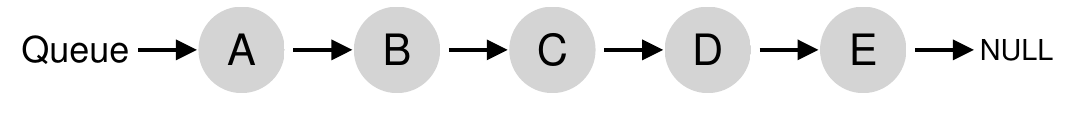
\includegraphics[width=1.\textwidth]{single-queue}
	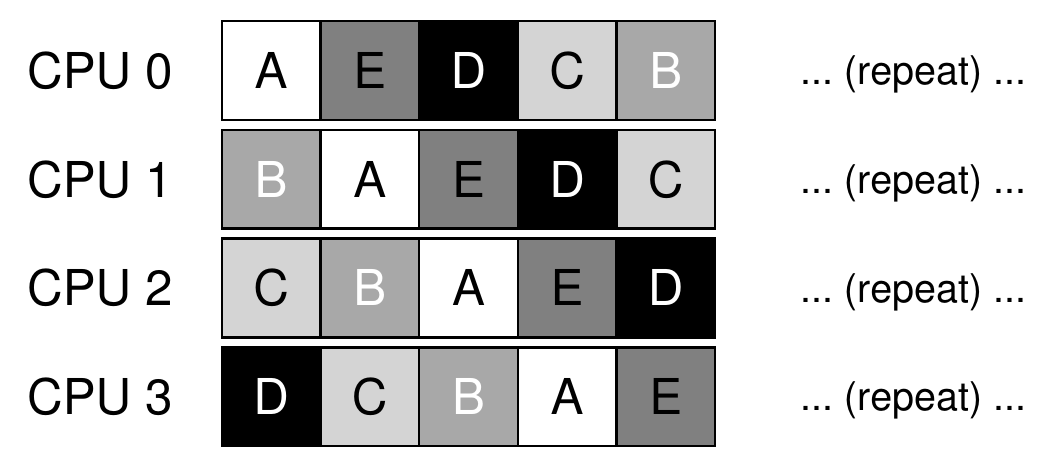
\includegraphics[width=1.\textwidth]{sqms}	
	\end{column}
	
	\begin{column}{.5\textwidth}
		% \large 单队列多处理器调度
    \begin{itemize}
        \item Single Queue Multiprocessor Scheduling,SQMS
        \item 简单地复用单处理器调度的基本架构
        \item 所有需要调度的进程放入 一个单独的队列中
    \end{itemize}

	\end{column}
\end{columns}
\end{frame}
%%------------------------------------------------
\begin{frame}
    \frametitle{单队列多处理器调度(SQMS)}	
	\begin{columns}
		\begin{column}{.5\textwidth}
			\Large \centering
			% 单队列调度
			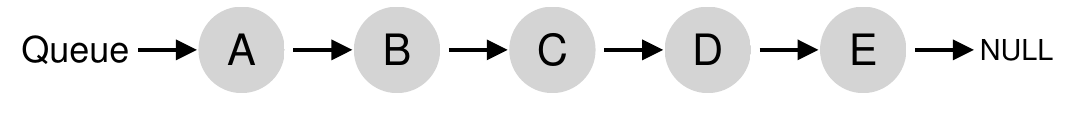
\includegraphics[width=1.\textwidth]{single-queue}
			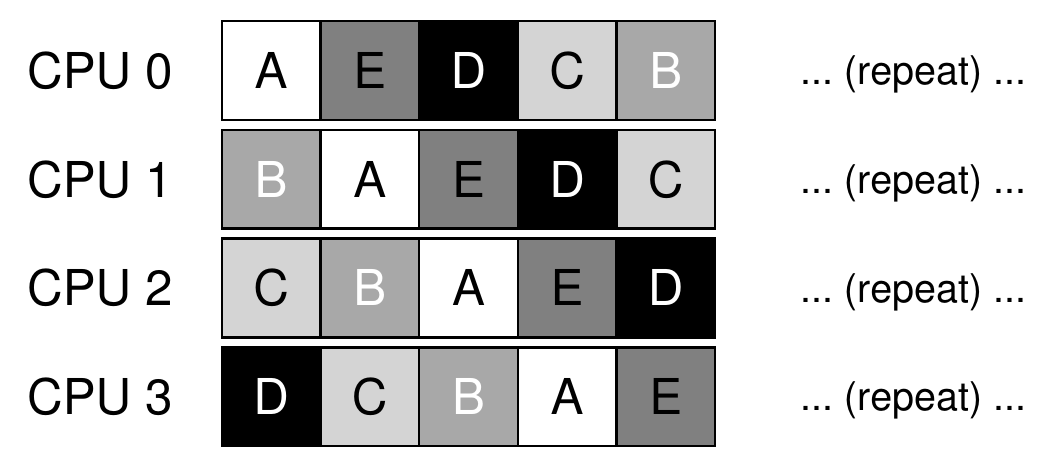
\includegraphics[width=1.\textwidth]{sqms}	
		\end{column}
		
		\begin{column}{.5\textwidth}
			\large
			单队列多处理器调度的缺点
			

			\begin{itemize}\large
				\item 缺乏可扩展性(scalability)
				\item 缓存亲和性(cache affinity)弱
			\end{itemize}
			
		\end{column}
	\end{columns}
\end{frame}


%%------------------------------------------------
\begin{frame}
    \frametitle{单队列多处理器调度(SQMS)}	
	\begin{columns}
		\begin{column}{.5\textwidth}
			\Large \centering
			% 单队列调度
			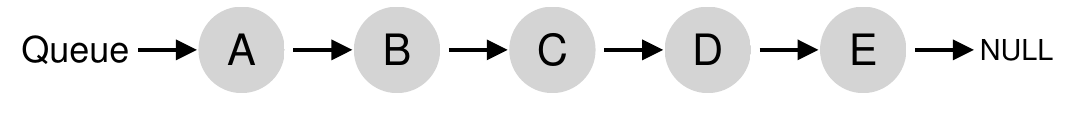
\includegraphics[width=1.\textwidth]{single-queue}
			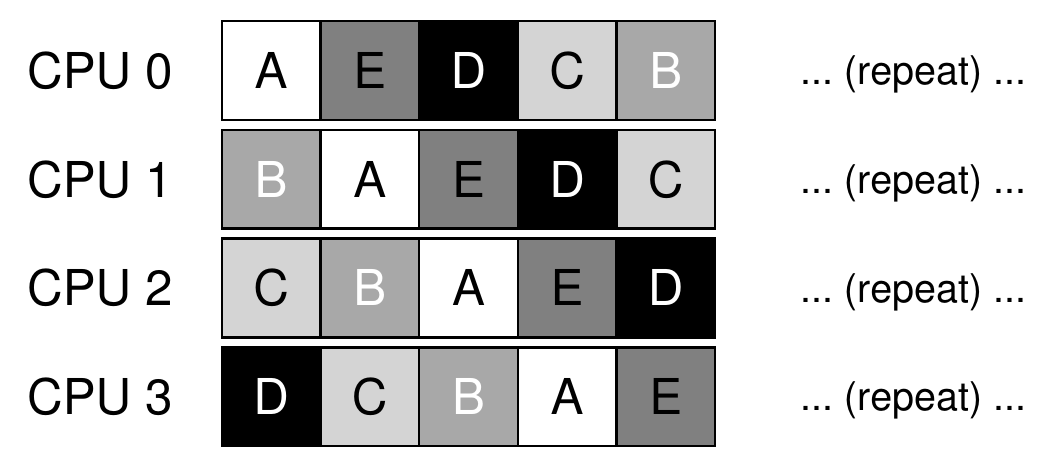
\includegraphics[width=1.\textwidth]{sqms}	
		\end{column}
		
		\begin{column}{.5\textwidth}
			\large
			% 单队列多处理器调度(SQMS) \\
			\normalsize
			尽可能让进程在同一个CPU上运行。保持一些进程的亲和度的同时,可能需要牺牲其他进程的亲和度来实现负载均衡。
			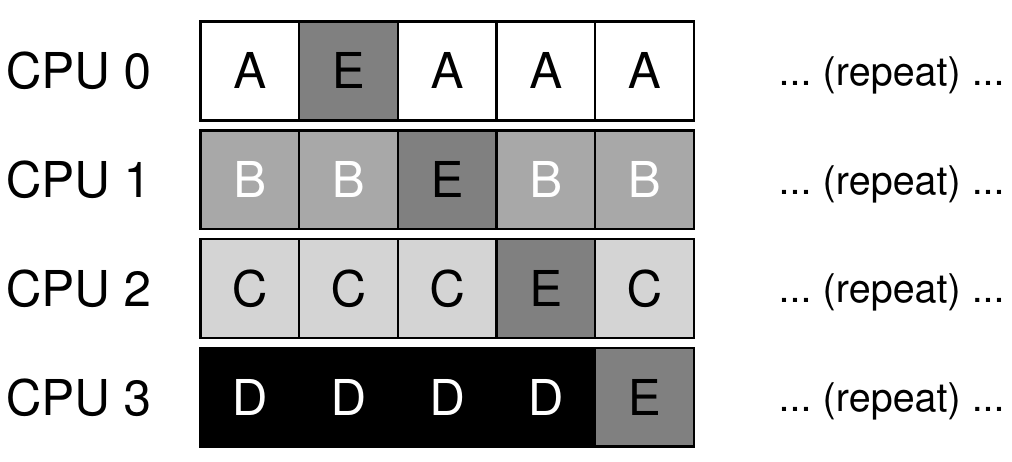
\includegraphics[width=1.\textwidth]{sqms-cache-affinity}

			
		\end{column}
	\end{columns}
\end{frame}

%%------------------------------------------------
\subsection{多队列多处理器调(MQMS)}
%----------------------------------------------
\begin{frame}
\frametitle{提纲} % Table of contents slide, comment this block out to remove it
\tableofcontents % Throughout your presentation, if you choose to use \section{} and \subsection{} commands, these will automatically be printed on this slide as an overview of your presentation

\end{frame}
%----------------------------------------------
\begin{frame}
    \frametitle{多队列多处理器调(MQMS)}
	\begin{columns}
		\begin{column}{.5\textwidth}
			\Large \centering
			% 多队列调度
			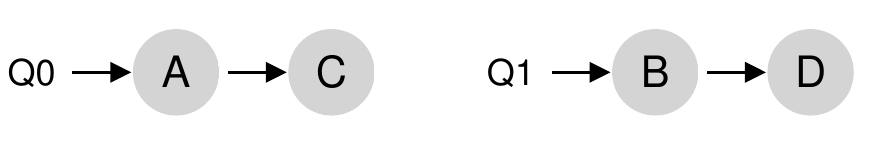
\includegraphics[width=1.\textwidth]{multi-queue}
			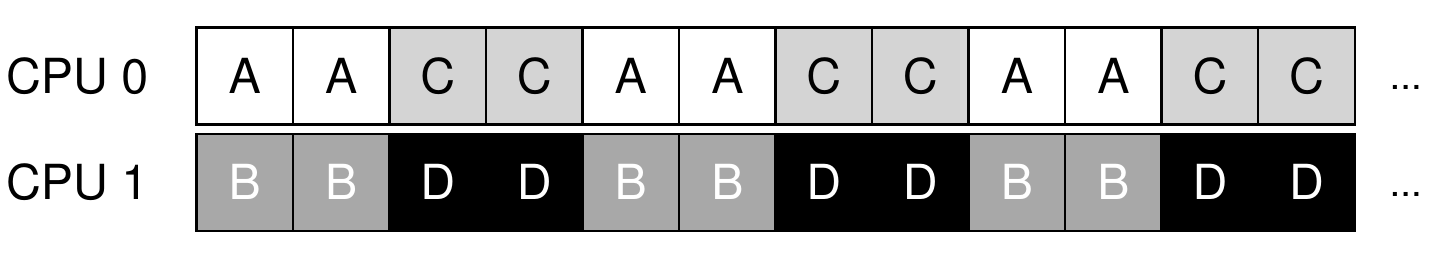
\includegraphics[width=1.\textwidth]{mqms}	
		\end{column}
		
		\begin{column}{.5\textwidth}
			% \large
			% 多队列多处理器调度 \\
			\normalsize
			\begin{itemize}
			\item Multi-Queue Multiprocessor Scheduling,MQMS
			\item 基本调度框架包含多个调度队列,每个队列可以使用不同的调度规则,比如轮转等算法。
			
			\item 进程进入系统时,依照 一些启发性规则(如随机或选择较空的队列)将其放入某个调度队列。
			\item 每个CPU调度相互独立,避免单队列方式的数据共享及同步问题。
			\end{itemize}
		\end{column}
	\end{columns}
\end{frame}


%%------------------------------------------------
\begin{frame}
    \frametitle{多队列多处理器调度(MQMS)的优点}
	\begin{columns}
		\begin{column}{.5\textwidth}
			\Large \centering
			% 多队列调度
			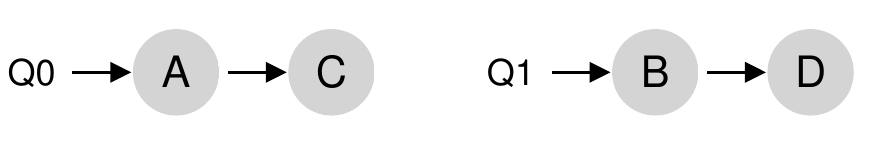
\includegraphics[width=1.\textwidth]{multi-queue}
			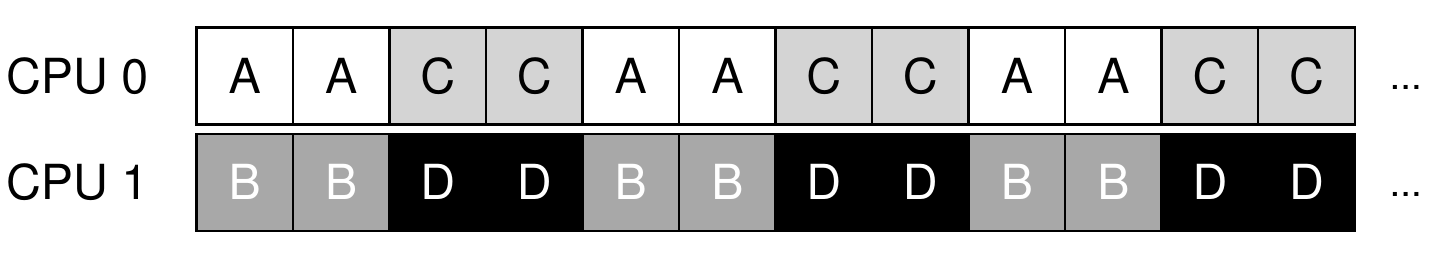
\includegraphics[width=1.\textwidth]{mqms}	
		\end{column}
		
		\begin{column}{.5\textwidth}
			\large
			% 多队列多处理器调度(MQMS) 
			\normalsize
			\begin{itemize}
			\item 根据不同队列的调度策略,每个CPU从两个进程中选择,决定谁将运行。例如,轮转调度
			\item 具有可扩展性:队列的数量会随着CPU的增加而增加,因此锁和缓存争用的开销不是大问题。
			\item 具有良好的缓存亲和度:所有进程都保持在固定的CPU上,因而可以很好地利用缓存数据。
			\end{itemize}
		\end{column}
	\end{columns}
\end{frame}


%%------------------------------------------------
\begin{frame}
    \frametitle{多队列多处理器调度的负载不均}
	\begin{columns}
		\begin{column}{.5\textwidth}
			\Large \centering
			%多队列调度
			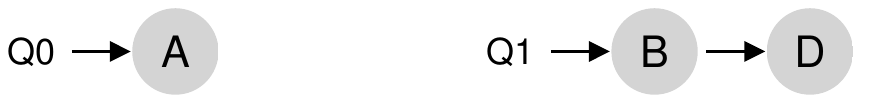
\includegraphics[width=1.\textwidth]{mqms-problem-1}
			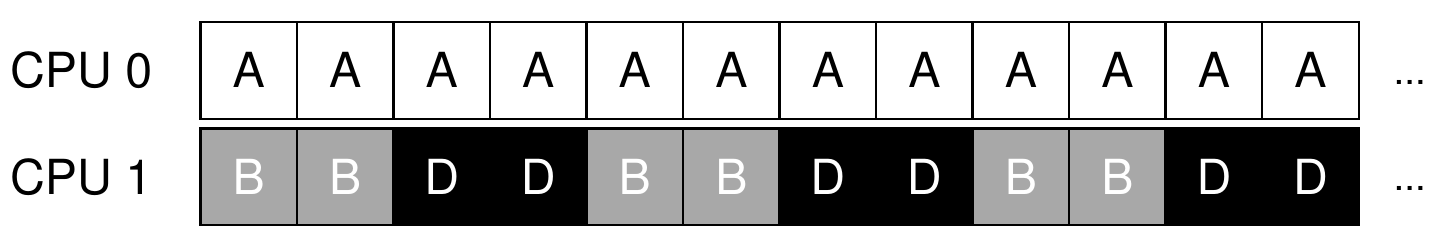
\includegraphics[width=1.\textwidth]{mqms-problem-2}	
		\end{column}
		
		\begin{column}{.5\textwidth}
			\large
			%MQMS的负载不均\\ 
			\normalsize
			
			\begin{itemize}
				\item 假定4个进程,2个CPU;队列都执行轮转调度策略;进程C执行完毕
			\item  A获得了B和D两倍的CPU时间

			\end{itemize}
		\end{column}
	\end{columns}
\end{frame}

%----------------------------------------------


%%------------------------------------------------
\begin{frame}
    \frametitle{多队列多处理器调度的负载不均}
	\begin{columns}
		\begin{column}{.5\textwidth}
			%\Large \centering
			%多队列调度
			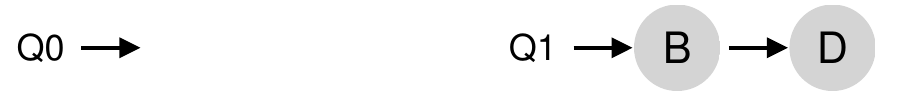
\includegraphics[width=1.\textwidth]{mqms-problem-3}
			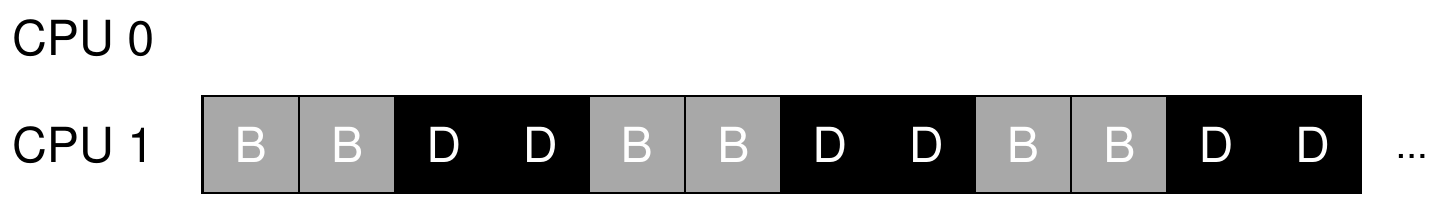
\includegraphics[width=1.\textwidth]{mqms-problem-4}	
		\end{column}
		
		\begin{column}{.5\textwidth}
			\large
			%MQMS的负载不均 \\
			\normalsize
			假定4个进程,2个CPU;每个队列都执行轮转调度策略;A和C都执行完毕,系统中只有B和D
			\begin{itemize}
				\item CPU1很忙
				\item CPU0空闲
				
			\end{itemize} \pause
		\Large
		怎样才能克服潜伏的负载不均问题?
		\end{column}
	\end{columns}
\end{frame}



%%------------------------------------------------
\subsection{多队列调度:工作窃取}
%----------------------------------------------
\begin{frame}
\frametitle{提纲} % Table of contents slide, comment this block out to remove it
\tableofcontents % Throughout your presentation, if you choose to use \section{} and \subsection{} commands, these will automatically be printed on this slide as an overview of your presentation

\end{frame}
%----------------------------------------------
\begin{frame}
	\frametitle{如何应对负载不均}
	\begin{columns}
		\begin{column}{.5\textwidth}
			\Large \centering
			%多队列调度
			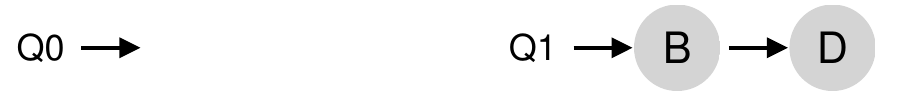
\includegraphics[width=1.\textwidth]{mqms-problem-3}
			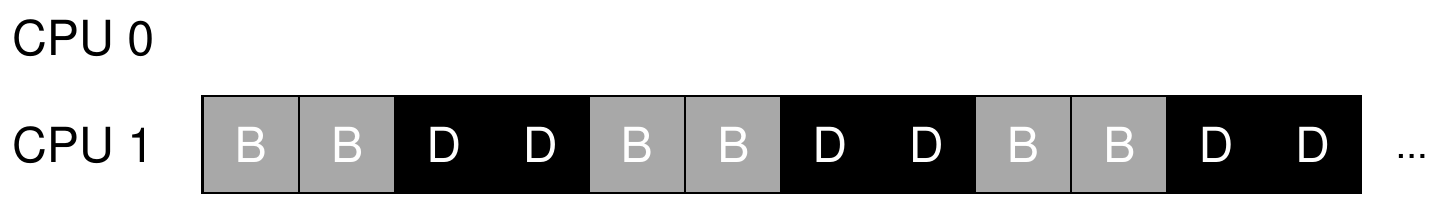
\includegraphics[width=1.\textwidth]{mqms-problem-4}	
		\end{column}
		
		\begin{column}{.5\textwidth}
%			\large
			\begin{block}{关键问题:如何应对负载不均}
			多队列多处理器调度程序应该如何处理负载不均问题,从而更好地实现预期的调度目标?
			\end{block} 
			\normalsize
			进程迁移(migration):通过进程的跨CPU迁移,可以真正实现负载均衡。 \pause
			
			\begin{itemize}
				\item 情况:有一个CPU空闲,另一个CPU有一些进程。
				\item 迁移:将B或D迁移到CPU0。
		
			\end{itemize}
			\Large

		\end{column}
	\end{columns}
\end{frame}



%%------------------------------------------------
\begin{frame}
	\frametitle{如何应对负载不均}
	\begin{columns}
		\begin{column}{.5\textwidth}
			\Large \centering
			% 多队列调度
			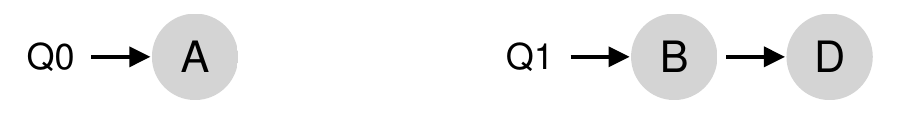
\includegraphics[width=1.\textwidth]{mqms-problem-5}
			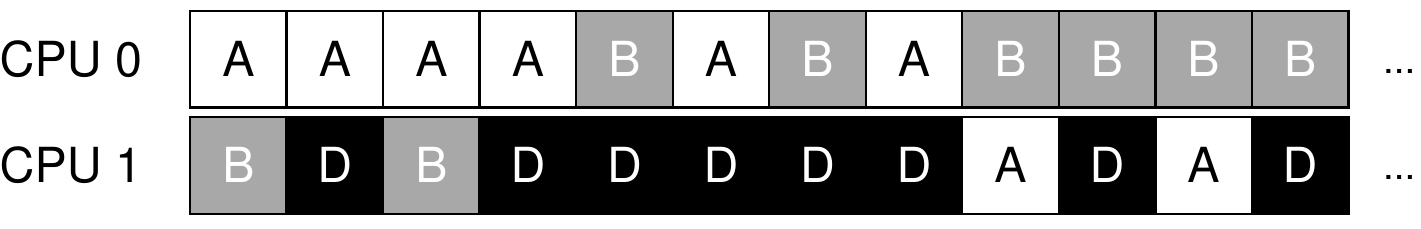
\includegraphics[width=1.\textwidth]{mqms-problem-6}	
		\end{column}
		
		\begin{column}{.5\textwidth}
%			\large
			\begin{block}{关键问题:如何应对负载不均}
			多队列多处理器调度程序应该如何处理负载不均问题,从而更好地实现预期的调度目标?
			\end{block} 
			\normalsize
			进程迁移(migration):通过进程的跨CPU迁移,可以真正实现负载均衡。 
			
			\begin{itemize}
				\item 情况:A独自留在CPU 0上,B和D在CPU 1上交替运行
				\item 迁移:不断地迁移和切换一个或多个进程

			\end{itemize} \pause
		\large
		系统如何决定发起这样的迁移?
			\Large
			
		\end{column}
	\end{columns}
\end{frame}



%%------------------------------------------------
\begin{frame}
	\frametitle{多队列调度:工作窃取(work stealing)}
	\begin{columns}
		\begin{column}{.5\textwidth}
			\Large \centering
			
			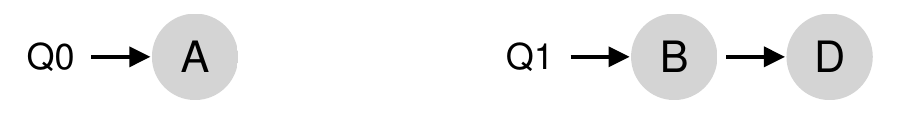
\includegraphics[width=1.\textwidth]{mqms-problem-5}
			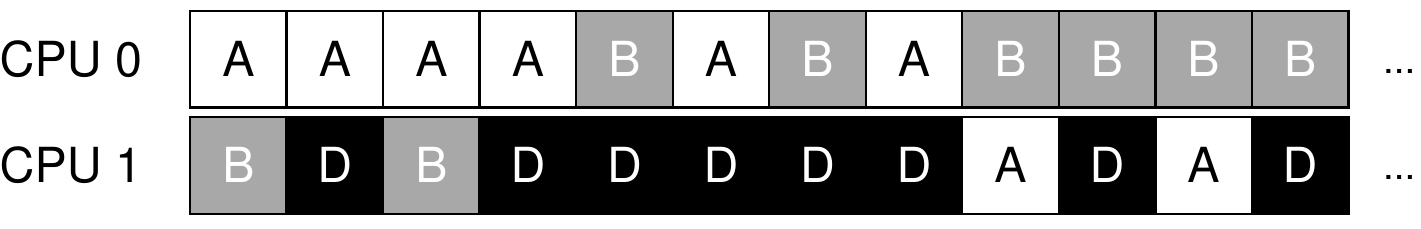
\includegraphics[width=1.\textwidth]{mqms-problem-6}	
			
			\normalsize
			
			\begin{itemize}
				\item 进程量较少的(源)队列不定期地“偷看”其他(目标)队列是不是比自己的进程多
				\item 如果目标队列比源队列 (显著地)更满,就从目标队列“窃取”一个或多个进程,实现负载均衡。
				
			\end{itemize}

		
		\end{column}
			\pause		
		\begin{column}{.5\textwidth}
%			\large
			工作窃取的队列检查间隔

			\normalsize
		
			\begin{itemize}
				\item 如果太频繁地检查其他队列,就会带来较高的开销,可扩展性不好
				\item 如果检查间隔太长,又可能会带来严重的负载不均
			\end{itemize}

			
		\end{column}
	\end{columns}
\end{frame}
%----------------------------------------------





\end{document}
